%\section{Table-based local store}

In GIGA+, we use a key-value store 
one instance of \ldb \citep{LevelDB} on each GIGA+ server.
This \ldb instance stores all inode attributes and the directory entries 
for one or more directories by this server.

\textbf{LevelDB -- }
Inspired by a simpler structure in BigTable\citep{BigTable}, LevelDB \citep{LevelDB} is an open-source key-value storage library
that features an Log-Structured Merge (LSM) Tree \citep{ONeil1996} for on-disk storage.
It provides simple APIs such as GET, PUT, DELETE and SCAN.
Unlike BigTable, not even single row transactions are supported in LevelDB. 

\begin{figure}[!ht]
\centering
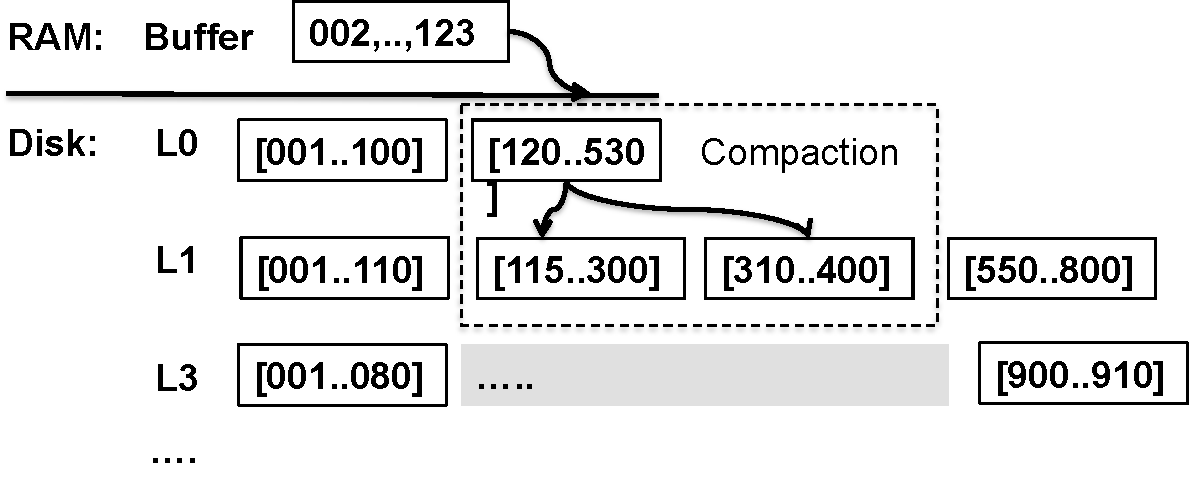
\includegraphics[scale=0.4]{figs/leveldb}
\caption{LevelDB represents data on disk in multiple SSTables that store sorted key-value pairs.}
\label{fig:leveldb}
\end{figure}

In a simple understanding of an LSM tree, an in memory buffer cache delays writing new and changed entries until it has a significant amount of change to record on disk. Delaying writes is made more durable by redundantly recording new and changed entries in a write-ahead log, which is pushed to disk periodically and asynchronously by default.

In LevelDB, by default, a set of changes are spilled to disk when the total size of modified entries exceeds 4 MB.  When a spill is triggered, called a minor compaction, the changed entries are sorted, indexed and written to disk in a format called an SSTable\citep{BigTable}.  These entries may then be discarded by the in memory buffer and can be reloaded by searching each SSTable on disk, possibly stopping when the first match occurs if the SSTables are searched most recent to oldest.  The number of SSTables that need to be searched can be reduced by maintaining a Bloom filter\citep{bloomfilter} on each, but with time the cost of finding a record not in memory increases.  Major compaction, or simply ``compaction", is the process of combining multiple SSTables into a smaller number of SSTables by merge sort. Compaction is similar to \emph{online defragmentation} in traditional file systems and \emph{cleaning} in log-structured file systems \citep{LFS}.

As illustrated in Figure \ref{fig:leveldb}, LevelDB extends this simple approach to further reduce read costs by dividing SSTables into sets, or levels.
The 0th level of SSTables follows the simple formulation; each SSTable in this level may contain entries with any key value, based on what was in memory at the time of its spill.
The higher levels of LevelDB's SSTables are the results of compacting SSTables from their own or lower levels.
In these higher levels, LevelDB maintains the following invariant: the key range spanning each SSTable is disjoint from the key range of all other SSTables at that level.
So querying for an entry in the higher levels only need read at most one SSTable in each level.
LevelDB also sizes each of the higher levels differentially:  all SSTables have the same maximum size and the sum of the sizes of all SSTables at level $L$ will not exceed $10^L$ MB.
This ensures that the number of level, that is, the maximum number of SSTables that need to be searched in the higher levels, grows logarithmically with increasing numbers of entries.

\textbf{Table Schema --}

\giga's metadata store aggregates directory entries, 
inode attributes and small files into one \ldb table with a row for each file.
To link together the hierarchical structure of the user's namespace,
the rows of the table are ordered by a 128-bit key consisting of 
the 64-bit inode number of a file's parent directory 
and a 64-bit hash value of its filename string (final component of its pathname).
The value of a row contains the file's full name and inode attributes,
such as inode number, ownership, access mode, file size, timestamps (\textit{struct stat} in Linux).
For small files, the file's row also contains the file's data.

Figure \ref{fig:schema} shows an example of storing a sample file system's metadata into one LevelDB table.
\begin{figure}[!ht]
\centering
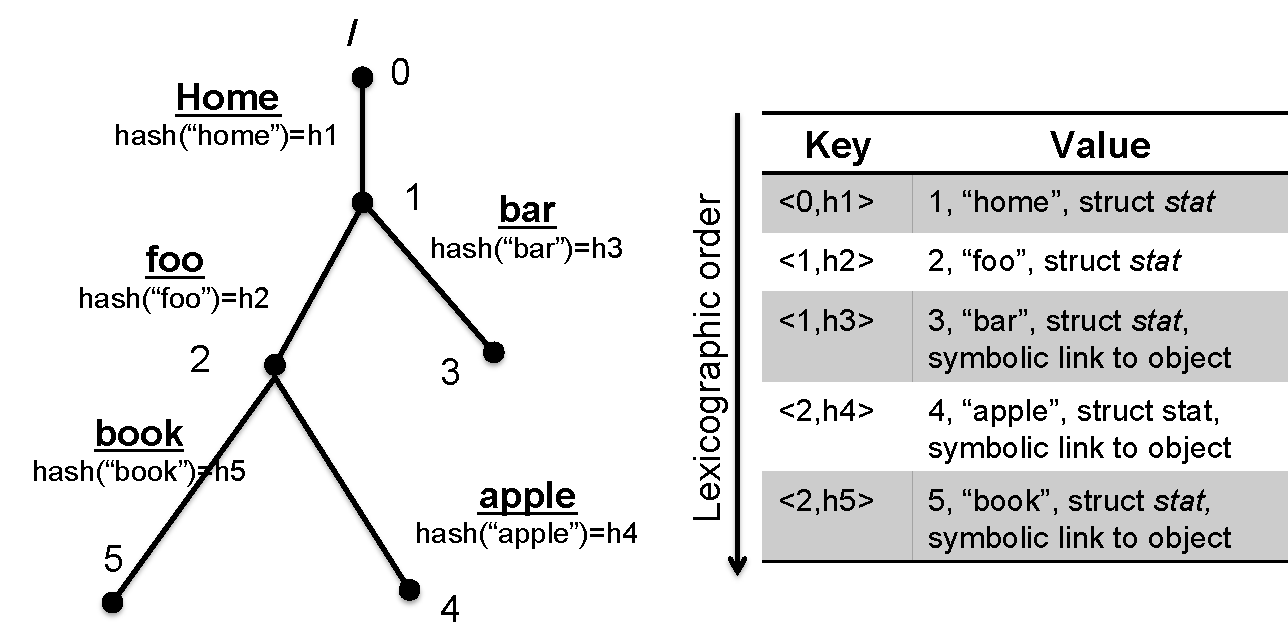
\includegraphics[scale=0.35]{figs/schema}
\caption{An example illustrates table schema used by \tfs's metadata store.
         The file with inode number 4 has two hard links,
         one called ``apple" from directory \textit{foo} and 
         the other called ``orange" from directory \textit{bar}.}
\label{fig:schema}
\end{figure}

All the entries in the same directory have rows that 
share the same first 64 bits in their the table's key.
For $readdir$ operations, once the inode number
of the target directory has been retrieved, 
a scan sequentially lists all entries having 
the directory's inode number as the first 64 bits of their table's key. 
To resolve a single pathname, \tfs starts searching from the root inode, 
which has a well-known inode number $(0)$.
Traversing the user's directory tree
involves constructing a search key by concatenating the inode 
number of current directory with the hash of
next component name in the pathname.
Unlike BTRFS, \tfs does not need the second version of each directory entry
because the entire attributes are returned in the \textit{readdir} scan.



